% questions.tex —— 2010 年·普通高等学校招生考试·广东卷·文科 · 题目内容片段（无答案）
% 由 tools/generate_projects.py 依来源总账自 2010/2010_数学真题_广东文_试题.md 生成，勿手改（改源 MD 后重跑）


状态：needs-review；依固定候选 PDF 两页（印刷页 595–596）逐题核验，五幅图已矢量重绘。原页未印分值，不补。

\gkpart{一、选择题}

\begin{question}
\gkti{1}若集合 $A=\{0,1,2,3\}$，$B=\{1,2,4\}$，则集合 $A\cup B=$（　）

（A）$\{0,1,2,3,4\}$

（B）$\{1,2,3,4\}$

（C）$\{1,2\}$

（D）$\{0\}$

\end{question}
\begin{question}
\gkti{2}函数 $f(x)=\lg(x-1)$ 的定义域是（　）

（A）$(2,+\infty)$

（B）$(1,+\infty)$

（C）$[1,+\infty)$

（D）$[2,+\infty)$

\end{question}
\begin{question}
\gkti{3}若函数 $f(x)=3^x+3^{-x}$ 与 $g(x)=3^x-3^{-x}$ 的定义域均为 $\mathbf R$，则（　）

（A）$f(x)$ 与 $g(x)$ 均为偶函数

（B）$f(x)$ 为奇函数，$g(x)$ 为偶函数

（C）$f(x)$ 与 $g(x)$ 均为奇函数

（D）$f(x)$ 为偶函数，$g(x)$ 为奇函数

\end{question}
\begin{question}
\gkti{4}已知数列 $\{a_n\}$ 为等比数列，$S_n$ 是它的前 $n$ 项和，若 $a_2\cdot a_3=2a_1$，且 $a_4$ 与 $2a_7$ 的等差中项为 $\dfrac54$，则 $S_5=$（　）

（A）$35$

（B）$33$

（C）$31$

（D）$29$

\end{question}
\begin{question}
\gkti{5}若向量 $\boldsymbol a=(1,1)$，$\boldsymbol b=(2,5)$，$\boldsymbol c=(3,x)$ 满足条件 $(8\boldsymbol a-\boldsymbol b)\cdot\boldsymbol c=30$，则 $x=$（　）

（A）$6$

（B）$5$

（C）$4$

（D）$3$

\end{question}
\begin{question}
\gkti{6}若圆心在 $x$ 轴上、半径为 $\sqrt5$ 的圆 $O$ 位于 $y$ 轴左侧，且与直线 $x+2y=0$ 相切，则圆 $O$ 的方程是（　）

（A）$(x-\sqrt5)^2+y^2=5$

（B）$(x+\sqrt5)^2+y^2=5$

（C）$(x-5)^2+y^2=5$

（D）$(x+5)^2+y^2=5$

\end{question}
\begin{question}
\gkti{7}若一个椭圆长轴的长度、短轴的长度和焦距成等差数列，则该椭圆的离心率是（　）

（A）$\frac45$

（B）$\frac35$

（C）$\frac25$

（D）$\frac15$

\end{question}
\begin{question}
\gkti{8}“$x>0$”是“$\sqrt[3]{x^2}>0$”的（　）

（A）充分非必要条件

（B）必要非充分条件

（C）非充分非必要条件

（D）充要条件

\Needspace{0.4\textheight}
\end{question}
\begingroup
\renewenvironment{question}{\Needspace{0.5\textheight}}{}
\begin{question}
\gkti{9}如图，$\triangle ABC$ 为正三角形，$AA'\parallel BB'\parallel CC'$，$CC'\perp$ 平面 $ABC$，且 $3AA'=\dfrac32BB'=CC'=AB$，则多面体 $ABC-A'B'C'$ 的正视图（也称主视图）是（　）
\nopagebreak[4]
\begin{center}% 2010 年广东卷文科第 9 题：多面体 ABC-A'B'C'。
% 来源 PDF：普通高考/2010/2010广东文.pdf，SHA-256 dd04b2053a22c854a9abe1ee03241fc04d5a25c91cda1d7997183bdfaa4a8c6f。
% 原页：第 1 页（A3 三栏）第 1 栏下部，书页码 595。
% 重绘依据：ABC 为正三角形；AA'、BB'、CC' 平行且 CC'⊥平面 ABC；
%   3AA'=(3/2)BB'=CC'=AB。AC 与 CC' 为不可见棱，画虚线。
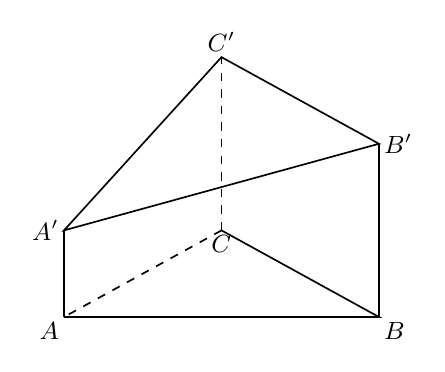
\begin{tikzpicture}[semithick, every node/.style={inner sep=1.6pt, font=\small}]
  \coordinate (A) at (0,0);
  \coordinate (B) at (4,0);
  \coordinate (C) at (2,1.1);
  \coordinate (Ap) at (0,1.1);
  \coordinate (Bp) at (4,2.2);
  \coordinate (Cp) at (2,3.3);

  \draw (A) -- (B) -- (C);
  \draw[dashed] (C) -- (A);
  \draw (A) -- (Ap);
  \draw (B) -- (Bp);
  \draw[dashed] (C) -- (Cp);
  \draw (Ap) -- (Bp) -- (Cp) -- cycle;

  \node[below left] at (A) {$A$};
  \node[below right] at (B) {$B$};
  \node[below] at (C) {$C$};
  \node[left] at (Ap) {$A'$};
  \node[right] at (Bp) {$B'$};
  \node[above] at (Cp) {$C'$};
\end{tikzpicture}
\end{center}
\nopagebreak[4]
\nopagebreak[4]
\begin{center}% 2010 年广东卷文科第 9 题选项图：四个正视图（A）—（D）。
% 来源 PDF：普通高考/2010/2010广东文.pdf，SHA-256 dd04b2053a22c854a9abe1ee03241fc04d5a25c91cda1d7997183bdfaa4a8c6f。
% 原页：第 1 页（A3 三栏）第 2 栏上部，书页码 595。
% 重绘依据：D 为正确视图：左端低、右端较高、中央最高且有中央虚线；
%   A、B、C 为干扰项（A 左高右低，B 单调上升，C 单调下降）。
\begin{tikzpicture}[semithick, scale=0.85, every node/.style={inner sep=1.2pt, font=\small}]
  % (A)
  \begin{scope}
    \draw (0,0) -- (3,0) -- (3,0.9) -- (1.5,2.1) -- (0,1.2) -- cycle;
    \draw[dashed] (1.5,0) -- (1.5,2.1);
    \node at (1.5,-0.55) {（A）};
  \end{scope}
  % (B)
  \begin{scope}[shift={(5,0)}]
    \draw (0,0) -- (3,0) -- (3,2.1) -- (0,0.9) -- cycle;
    \draw (0,0.9) -- (3,1.2);
    \node at (1.5,-0.55) {（B）};
  \end{scope}
  % (C)
  \begin{scope}[shift={(10,0)}]
    \draw (0,0) -- (3,0) -- (3,1.2) -- (0,2.1) -- cycle;
    \draw (0,1.2) -- (3,0.9);
    \node at (1.5,-0.55) {（C）};
  \end{scope}
  % (D)
  \begin{scope}[shift={(15,0)}]
    \draw (0,0) -- (3,0) -- (3,1.5) -- (1.5,2.1) -- (0,0.6) -- cycle;
    \draw[dashed] (1.5,0) -- (1.5,2.1);
    \node at (1.5,-0.55) {（D）};
  \end{scope}
\end{tikzpicture}
\end{center}
\nopagebreak[4]
\end{question}
\endgroup
\begin{question}
\gkti{10}在集合 $\{a,b,c,d\}$ 上定义两种运算 $\oplus$ 和 $\otimes$ 如下：

\nopagebreak[4]
\[
\begin{array}{c|cccc}
\oplus & a & b & c & d\\\hline
a & a & b & c & d\\
b & b & b & b & b\\
c & c & b & c & b\\
d & d & b & b & d
\end{array}
\qquad
\begin{array}{c|cccc}
\otimes & a & b & c & d\\\hline
a & a & a & a & a\\
b & a & b & c & d\\
c & a & c & c & a\\
d & a & d & a & d
\end{array}
\]

那么 $d\otimes(a\oplus c)=$（　）

（A）$a$

（B）$b$

（C）$c$

（D）$d$

\end{question}
\gkpart{二、填空题}

\Needspace{0.4\textheight}
\begingroup
\renewenvironment{question}{\Needspace{0.5\textheight}}{}
\begin{question}
\gkti{11}某城市缺水问题比较突出，为了制定节水管理办法，对全市居民某年的月均用水量进行了抽样调查，其中 $4$ 位居民的月均用水量分别为 $x_1,\cdots,x_4$（单位：吨）。根据如图所示的程序框图，若 $x_1,x_2,x_3,x_4$ 分别为 $1,1.5,1.5,2$，则输出的结果 $s$ 为$\underline{\qquad}$。
\nopagebreak[4]
\begin{center}% 2010 年广东卷文科第 11 题：程序框图。
% 来源 PDF：普通高考/2010/2010广东文.pdf，SHA-256 dd04b2053a22c854a9abe1ee03241fc04d5a25c91cda1d7997183bdfaa4a8c6f。
% 原页：第 1 页（A3 三栏）第 2 栏中部，书页码 595。
% 重绘依据：开始 → 输入 x1..x4 → s1=0,i=1 → 判断 i≤4；
%   是（右）→ s1=s1+xi → s=(1/i)s1 → i=i+1 → 回到判断前；
%   否（下）→ 输出 s → 结束。
\begin{tikzpicture}[semithick, >=Stealth,
  every node/.style={inner sep=1.5pt, font=\small}]
  \node (start) [draw, rounded corners=4pt, minimum width=1.8cm, minimum height=0.55cm] at (0,0) {开始};
  \node (in) [draw, trapezium, trapezium left angle=72, trapezium right angle=108,
    minimum width=3.2cm, minimum height=0.55cm] at (0,-1.4) {输入 $x_1,\cdots,x_4$};
  \node (init) [draw, minimum width=2.8cm, minimum height=0.6cm] at (0,-3.0) {$s_1=0$，$i=1$};
  \node (test) [draw, diamond, aspect=2.2, minimum width=2.8cm, minimum height=1.15cm] at (0,-4.9) {$i\leqslant4$};
  \node (out) [draw, trapezium, trapezium left angle=72, trapezium right angle=108,
    minimum width=2.2cm, minimum height=0.55cm] at (0,-6.9) {输出 $s$};
  \node (end) [draw, rounded corners=4pt, minimum width=1.8cm, minimum height=0.55cm] at (0,-8.2) {结束};
  \node (add) [draw, minimum width=2.4cm, minimum height=0.6cm] at (4.4,-3.8) {$s_1=s_1+x_i$};
  \node (avg) [draw, minimum width=2.2cm, minimum height=0.65cm] at (4.4,-2.7) {$s=\dfrac1i s_1$};
  \node (inc) [draw, minimum width=1.5cm, minimum height=0.55cm] at (4.4,-1.65) {$i=i+1$};

  \draw[->] (start) -- (in);
  \draw[->] (in) -- (init);
  \draw[->] (init) -- (test);
  \draw[->] (test.south) -- node[right] {否} (out.north);
  \draw[->] (out) -- (end);
  \draw[->] (test.east) -- node[above] {是} (add.west);
  \draw[->] (add) -- (avg);
  \draw[->] (avg) -- (inc);
  \draw[->] (inc.north) -- (4.4,-0.75) -- (-3.8,-0.75) -- (-3.8,-3.0) -- (init.west);
\end{tikzpicture}
\end{center}
\nopagebreak[4]
\end{question}
\endgroup
\begin{question}
\gkti{12}某市居民 $2005-2009$ 年家庭年平均收入 $x$（单位：万元）与年平均支出 $Y$（单位：万元）的统计资料如下表所示：

\begin{center}
\begin{tabular}{lrrrrr}
\toprule
年份 & $2005$ & $2006$ & $2007$ & $2008$ & $2009$ \\
\midrule
收入 $x$ & $11.5$ & $12.1$ & $13$ & $13.3$ & $15$ \\
支出 $Y$ & $6.8$ & $8.8$ & $9.8$ & $10$ & $12$ \\
\bottomrule
\end{tabular}
\end{center}

根据统计资料，居民家庭年平均收入的中位数是$\underline{\qquad}$，家庭年平均收入与年平均支出有$\underline{\qquad}$（填“正”或“负”）线性相关关系。

\end{question}
\begin{question}
\gkti{13}已知 $a,b,c$ 分别是 $\triangle ABC$ 的三个内角 $A,B,C$ 所对的边。若 $a=1$，$b=\sqrt3$，$A+C=2B$，则 $\sin A=$ $\underline{\qquad}$。

\Needspace{0.4\textheight}
\end{question}
\begingroup
\renewenvironment{question}{\Needspace{0.5\textheight}}{}
\begin{question}
\gkti{14}如图，在直角梯形 $ABCD$ 中，$DC\parallel AB$，$CB\perp AB$，$AB=AD=a$，$CD=\dfrac a2$，点 $E,F$ 分别为线段 $AB,AD$ 的中点，则 $EF=$ $\underline{\qquad}$。
\nopagebreak[4]
\begin{center}% 2010 年广东卷文科第 14 题：直角梯形 ABCD。
% 来源 PDF：普通高考/2010/2010广东文.pdf，SHA-256 dd04b2053a22c854a9abe1ee03241fc04d5a25c91cda1d7997183bdfaa4a8c6f。
% 原页：第 1 页（A3 三栏）第 3 栏中部，书页码 595。
% 重绘依据：A(0,0)、B(4,0)、C(4,3.46)、D(2,3.46)；E 为 AB 中点，F 为 AD 中点。
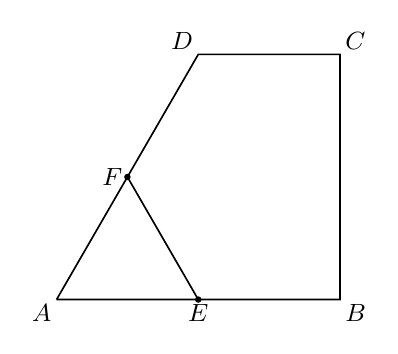
\begin{tikzpicture}[semithick, scale=0.9, every node/.style={inner sep=1.6pt, font=\small}]
  \coordinate (A) at (0,0);
  \coordinate (B) at (4,0);
  \coordinate (C) at (4,3.46);
  \coordinate (D) at (2,3.46);
  \coordinate (E) at (2,0);
  \coordinate (F) at (1,1.73);

  \draw (A) -- (B) -- (C) -- (D) -- (A);
  \draw (E) -- (F);
  \fill (E) circle (1.3pt);
  \fill (F) circle (1.3pt);
  \node[below left] at (A) {$A$};
  \node[below right] at (B) {$B$};
  \node[above right] at (C) {$C$};
  \node[above left] at (D) {$D$};
  \node[below] at (E) {$E$};
  \node[left] at (F) {$F$};
\end{tikzpicture}
\end{center}
\nopagebreak[4]
\end{question}
\endgroup
\begin{question}
\gkti{15}在极坐标系 $(\rho,\theta)$（$0\leqslant\theta<2\pi$）中，曲线 $\rho(\cos\theta+\sin\theta)=1$ 与 $\rho(\sin\theta-\cos\theta)=1$ 的交点的极坐标为$\underline{\qquad}$。

\end{question}
\gkpart{三、解答题}

\begin{question}
\gkti{16}设函数 $f(x)=3\sin\left(\omega x+\dfrac\pi6\right)$，$\omega>0$，$x\in(-\infty,+\infty)$，且以 $\dfrac\pi2$ 为最小正周期。

（1）求 $f(0)$；

（2）求 $f(x)$ 的解析式；

（3）已知 $f\left(\dfrac\alpha4+\dfrac\pi{12}\right)=\dfrac95$，求 $\sin\alpha$ 的值。

\end{question}
\begin{question}
\gkti{17}某电视台在一次对收看文艺节目和新闻节目观众的抽样调查中，随机抽取了 $100$ 名电视观众，相关的数据如下表所示：

\begin{center}
\begin{tabular}{lrrr}
\toprule
 & 文艺节目 & 新闻节目 & 总计 \\
\midrule
$20$ 到 $40$ 岁 & $40$ & $18$ & $58$ \\
大于 $40$ 岁 & $15$ & $27$ & $42$ \\
总计 & $55$ & $45$ & $100$ \\
\bottomrule
\end{tabular}
\end{center}

（1）由表中数据直观分析，收看新闻节目的观众是否与年龄有关？

（2）用分层抽样方法在收看新闻节目的观众中随机抽取 $5$ 名，大于 $40$ 岁的观众应该抽取几名？

（3）在上述抽取的 $5$ 名观众中任取 $2$ 名，求恰有 $1$ 名观众的年龄为 $20$ 至 $40$ 岁的概率。

\Needspace{0.4\textheight}
\end{question}
\begingroup
\renewenvironment{question}{\Needspace{0.5\textheight}}{}
\begin{question}
\gkti{18}如图，$\overset{\frown}{AEC}$ 是半径为 $a$ 的半圆，$AC$ 为直径，点 $E$ 为 $\overset{\frown}{AC}$ 的中点，点 $B$ 和点 $C$ 为线段 $AD$ 的三等分点，平面 $AEC$ 外一点 $F$ 满足 $FC\perp$ 平面 $BED$，$FB=\sqrt5a$。

（1）证明：$EB\perp FD$；

（2）求点 $B$ 到平面 $FED$ 的距离。
\nopagebreak[4]
\begin{center}% 2010 年广东卷文科第 18 题：半圆 AEC 与三棱锥 F-BED。
% 来源 PDF：普通高考/2010/2010广东文.pdf，SHA-256 dd04b2053a22c854a9abe1ee03241fc04d5a25c91cda1d7997183bdfaa4a8c6f。
% 原页：第 2 页（A3 三栏）第 1 栏上部，书页码 596。
% 重绘依据：A、B、C、D 共线且 AB=BC=CD；半圆以 AC 为直径、E 为弧中点；
%   F 在 C 上方，FC⊥平面 BED。FC、FB 为不可见棱，画虚线。
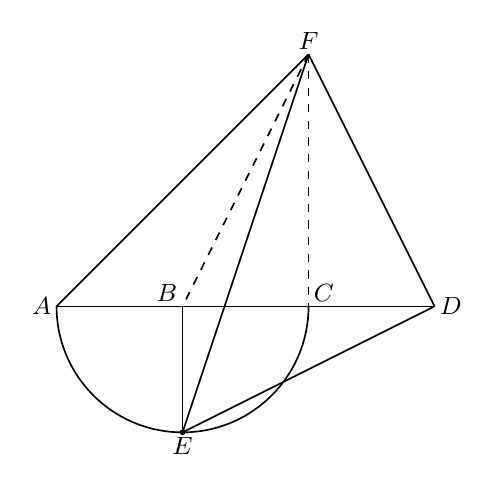
\begin{tikzpicture}[semithick, scale=0.8, every node/.style={inner sep=1.6pt, font=\small}]
  \coordinate (A) at (-2,0);
  \coordinate (B) at (0,0);
  \coordinate (C) at (2,0);
  \coordinate (D) at (4,0);
  \coordinate (E) at (0,-2);
  \coordinate (F) at (2,4);

  \draw (A) -- (D);
  \draw (A) arc[start angle=180,end angle=360,radius=2];
  \draw (F) -- (A);
  \draw (F) -- (D);
  \draw (F) -- (E);
  \draw[dashed] (F) -- (B);
  \draw[dashed] (F) -- (C);
  \draw (E) -- (B);
  \draw (E) -- (D);

  \fill (E) circle (1.3pt);
  \node[left] at (A) {$A$};
  \node[above left] at (B) {$B$};
  \node[above right] at (C) {$C$};
  \node[right] at (D) {$D$};
  \node[below] at (E) {$E$};
  \node[above] at (F) {$F$};
\end{tikzpicture}
\end{center}
\nopagebreak[4]
\end{question}
\endgroup
\begin{question}
\gkti{19}某营养师要为某个儿童预定午餐和晚餐。已知一个单位的午餐含 $12$ 个单位的碳水化合物，$6$ 个单位的蛋白质和 $6$ 个单位的维生素 C；一个单位的晚餐含 $8$ 个单位的碳水化合物，$6$ 个单位的蛋白质和 $10$ 个单位的维生素 C。另外，该儿童这两餐需要的营养中至少含 $64$ 个单位的碳水化合物，$42$ 个单位的蛋白质和 $54$ 个单位的维生素 C。如果一个单位的午餐、晚餐的费用分别是 $2.5$ 元和 $4$ 元，那么要满足上述的营养要求，并且花费最少，应当为该儿童分别预订多少个单位的午餐和晚餐？

\end{question}
\begin{question}
\gkti{20}已知函数 $f(x)$ 对任意实数 $x$ 均有 $f(x)=kf(x+2)$，其中常数 $k$ 为负数，且 $f(x)$ 在区间 $[0,2]$ 上有表达式 $f(x)=x(x-2)$。

（1）求 $f(-1)$，$f(2.5)$ 的值；

（2）写出 $f(x)$ 在 $[-3,3]$ 上的表达式，并讨论函数 $f(x)$ 在 $[-3,3]$ 上的单调性；

（3）求出 $f(x)$ 在 $[-3,3]$ 上的最小值与最大值，并求出相应的自变量的取值。

\end{question}
\begin{question}
\gkti{21}已知曲线 $C_n:y=nx^2$，点 $P_n(x_n,y_n)$（$x_n>0$，$y_n>0$）是曲线 $C_n$ 上的点（$n=1,2,\cdots$）。

（1）试写出曲线 $C_n$ 在点 $P_n$ 处的切线 $l_n$ 的方程，并求出 $l_n$ 与 $y$ 轴的交点 $Q_n$ 的坐标；

（2）若原点 $O(0,0)$ 到 $l_n$ 的距离与线段 $P_nQ_n$ 的长度之比取得最大值，试求点 $P_n$ 的坐标 $(x_n,y_n)$；

\Needspace{5\baselineskip}
（3）设 $m$ 与 $k$ 为两个给定的不同的正整数，$x_n$ 与 $y_n$ 是满足（2）中条件的点 $P_n$ 的坐标，证明：

\nopagebreak[4]
\[\sum_{n=1}^s\left|\sqrt{\frac{(m+1)x_n}{2}}-\sqrt{(k+1)y_n}\right|<\left|\sqrt{ms}-\sqrt{ks}\right|\quad(s=1,2,\cdots).\]

\end{question}